%%%%%%%%%%%%%%%%%%%%%%%%%%%%%%%%%%%%%%%%%%%%%%%%
% COPYRIGHT: (C) 2012-2015 FAU FabLab and others
% Bearbeitungen ab 2015-02-20 fallen unter CC-BY-SA 3.0
% Sobald alle Mitautoren zugestimmt haben, steht die komplette Datei unter CC-BY-SA 3.0. Bis dahin ist der Lizenzstatus aller alten Bestandteile ungeklärt.
%%%%%%%%%%%%%%%%%%%%%%%%%%%%%%%%%%%%%%%%%%%%%%%%


\newcommand{\basedir}{fablab-document}
\documentclass{\basedir/fablab-document}

\usepackage{amssymb} % Symbole für Knöpfe
\usepackage{subfigure,caption}
\usepackage{eurosym}
\usepackage{tabularx} % Tabellen mit bestimmtem Breitenverhältnis der Spalten
\usepackage{wrapfig} % Textumlauf um Bilder
\usepackage{float} % Ermöglicht H als Platzierungsoption
\renewcommand{\texteuro}{\euro}
\newcommand{\fachbegriff}[1]{(\textit{#1})}

% \linespread{1.2}
% \fancyhead{}
\date{\today}
\author{kontakt@fablab.fau.de}
\title{Einweisung 3D-Drucker}

\begin{document}

\maketitle
\begin{center}
	Für die 3D-Drucker \textbf{Makerbot Replicator 2X} und den \textbf{Ultimaker Original}
\end{center}

\textbf{Nur eingewiesene Benutzer dürfen den Drucker selbstständig benutzen}, um teure Beschädigungen zu vermeiden. Wenn du noch nicht eingewiesen bist, frage einen Betreuer. Er erklärt dir die Bedienung und lässt dich unter Aufsicht dein gewünschtes Teil ausdrucken. Wenn du alles verstanden hast, darfst auch du dann die Einweisung unterschreiben und den Drucker in Zukunft selbstständig verwenden.

\section{Regeln und Hinweise}
% Hier sollte nur das wichtigste gegen "Kaputtmachen" des Druckers stehen.
Für die Benutzung ist es wichtig, dass du folgende Hinweise beachtest:

\begin{itemize}
 \item Obwohl das 3D-Drucken unter den Begriff ``Rapid Prototyping'' fällt, kann ein Druck je nach Größe und 
 Präzision gut mehrere Stunden dauern. Betreuer helfen dir, die Dauer abzuschätzen. 
 \item Nicht unbeaufsichtigt drucken, immer wieder mal einen Blick darauf werfen, besonders am Anfang.\\
Wenn du nicht bis zum Ende deines Drucks da sein kannst, frage vorher einen Betreuer und hinterlasse einen Zettel mit Name und Kontaktdaten.
 \item Anleitung exakt beachten, wenn du nicht ganz genau weißt was du tust.\\
Wenn du nicht weiter weißt oder dir unsicher bist, frag einen Betreuer.
 \item Verbrennungsgefahr an heißen Teilen:
  \begin{itemize}
   \item Bodenplatte des Replicators wird knallheiß. Erst vorsichtig testen und evtl. Temperatur vorher absenken.
   \item Extruder wird sehr heiß! Nicht direkt berühren, Vorsicht beim Abputzen.
  \end{itemize}
 \item Drucker ausschalten,
 \begin{itemize}
  \item wenn der Drucker groben Unfug oder sehr seltsame Geräusche macht
  \item wenn der Drucker nicht mehr benötigt wird
  \item Replicator hinten rechts am Gehäuse, beim Ultimaker vorne am Gehäuse den Power-Switch betätigen
 \end{itemize}
 \item Wenn die Folie auf der Plattform beschädigt ist, bitte einen Betreuer es zu wechseln.
 \item \textbf{Keinen Schaber, Messer oder Ähnliches} verwenden, um Objekte von der Plattform zu lösen, denn dies beschädigt die Folie.
 \item am Drucker nichts von Hand bewegen ($\to$ \ref{manuelles-verfahren} Manuelles Verfahren auf Seite\, \pageref{manuelles-verfahren})
 \item Materialwechsel und sonstige Wartung darf nur gemeinsam mit einem Betreuer durchgeführt werden.
 \item \textbf{Wiegen und Bezahlen nicht vergessen!}
\end{itemize}
\newpage
\renewcommand{\contentsname}{Inhaltsverzeichnis / Arbeitsablauf}
\setcounter{tocdepth}{2}
\tableofcontents

\newpage

% % % % % % % % % % % % % % % %
\section{3D-Modell erstellen}
\subsection{Dateiformat}

Im STL-Dateiformat, Einheit: Millimeter. Alle gängigen 3D-Programme haben einen STL-Export.

\begin{itemize}
\item auf thingiverse.com gibt es viele vorgefertigte Modelle, als
Grundlage oder gleich zum fertig ausdrucken.
\item oder erstelle es mit einem Programm deiner Wahl
\begin{table}[H]
\centering
\begin{tabularx}{\textwidth}{|l|X|}
\hline \textbf{Name} & \textbf{Beschreibung} \\
\hline \textit{kostenlose Software} &  \\ 
\hline Blender & relativ komplex aber auch für Freiformflächen geeignet  \\ 
\hline OpenSCAD & Skriptsprache für Konstruktion aus geometrischen Grundkörpern \\ 
\hline DesignSpark Mechanical & Angelehnt an professionelle CAD-Software, aber relativ einfach zu bedienen  \\ 
\hline TinkerCAD & sehr einfach, für Kinder gut geeignet  \\ 
\hline Google SketchUp & wenig Einarbeitung, geringer Funktionsumfang, für einfache Teile \\
\hline & \\
\hline \textit{kostenpflichtige Software} & \\
\hline PTC Creo, Solid Edge, Siemens NX & kostenlos beim RRZE für Studenten, professionelle Software \\
\hline Autocad Inventor & kostenlos bei Autodesk für Studenten ebenfalls für professionelle Anwendungen \\
\hline 
\end{tabularx} 
\end{table}
\item Die 3D-Daten müssen gewisse Regeln erfüllen. Bei Modellierungsprogrammen wie Blender ist etwas Vorsicht oder Nacharbeit nötig, die meisten Konstruktionsprogramme (Solid Edge und Konsorten, auch OpenSCAD) machen es prinzipbedingt von selber richtig. Zu den Einschränkungen bei Blender stehen am Ende der Anleitung noch weitere Informationen.
\end{itemize}

\subsection{Einschränkungen der Formen}
\begin{itemize}
\item \textbf{Maximale Abmessungen} 
\begin{itemize}
 \item Makerbot: L:250 B:160 H:150mm
 \item Ultimaker: L:210 B:210 H:205mm
 \item zur Sicherheit lieber ein paar Millimeter kleiner.
 \item Es ist in der Praxis meist nicht möglich, den Bauraum des Druckers auch nur annähernd auszunutzen! Wenn möglich, gestalte deine Objekte kleiner als 10x10x5cm (LxBxH).
\end{itemize}
\item große Teile dauern ewig, während des Drucks muss jemand dabeibleiben. Druckzeit für 30x30x30mm sind je 
nach Präzision etwa 30-45 Minuten, ein größeres Volumen braucht entsprechend länger.
\item Durch das Druckverfahren gibt es gewisse Formen, die sich schlecht drucken lassen. Theoretisch ist fast
alles möglich, praktisch ist oft Ausprobieren angesagt. 
\item Damit man auch \enquote{schwierige} Formen drucken kann, kann die Software Stützstrukturen erstellen. Wenn man Stützstruktur anschaltet,
erzeugt der Drucker ein loses Geflecht unter Überhängen und Brücken,
das sich nach dem Ausdrucken mit einer Zange oder einem Skalpell entfernen lässt. So kann
man diese Begrenzungen umgehen. Nachteil ist die schlechtere
Oberflächenqualität und der Aufwand durch die mechanische
Nachbearbeitung.
\end{itemize}

\subsubsection{Drucken ohne Stützstruktur}
In diesem Abschnitt wird kurz beschrieben, welche Formen sich besonders gut drucken lassen, auch ohne Stützstruktur. Wenn es ohne großen Aufwand möglich ist, sollte man seine Konstruktionen gleich so wählen, dass sie gut druckbar sind.
\begin{center}
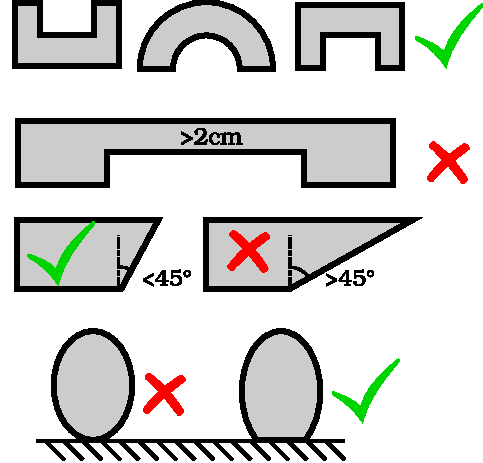
\includegraphics{./zeichnungen/formen.pdf}
\end{center}
\begin{itemize}
\item Überhänge sollten nicht zu groß sein
(Empfehlung {\textless}45°)
\item Brücken sollten nicht zu weit sein (Empfehlung {\textless}5mm)
\item Das Objekt sollte mit ausreichend großer Fläche plan auf dem Boden aufliegen
\item Der untere Teil des Objekts sollte immer eine stabile Unterlage für die darüberliegenden Schichten bilden. (Den Eiffelturm sollte man also nicht auf dem Kopf stehend drucken.)
\end{itemize}

% % % % % % % % % % % %
\section{Vorbereitung}

\subsection{Putzen} \label{putzen}
\begin{itemize}
 \item Bodenplatte mit Papiertuch und Oberflächenreiniger reinigen
 \item Extruderdüse ebenfalls mit Papiertuch reinigen
 \item \textbf{VORSICHT EVENTUELL HEIß!}
\end{itemize}

Wenn die Sorte bekannt ist, sortenreinen Kunststoffabfall in den entsprechend beschrifteten Behälter zum Recycling geben. Gemischte, verdreckte oder unbekannte Kunststoffreste bitte in den Restmüll.

\todoUnwichtig{welche Behälter} \todoUnwichtig{wann muss geputzt werden}

\subsection{Vorheizen}
Vorheizen ist normalerweise nicht nötig, da es automatisch vor dem Druck geschieht ($\to$ Kapitel \ref{vorheizen}).

\subsection{Material auswählen - PLA vs. ABS}
Grunsätzlich lässt sich PLA etwas einfacher und besser verarbeiten als ABS. Für ABS beötigt man z.B. eine beheiztes
Bett, das im Ultimaker nicht vorhanden ist. Mit PLA tut sich der Replicator dafür schwerer. Für die meisten 
Anwendungen ist es egal welches Material man verwendet, die Entscheidung richtet sich mehr nach der persönlichen
Vorliebe. Im Internet lässt sich einiges zu diesem Thema finden.

\subsubsection{PLA}
\begin{itemize}
\item Organisches Material, Biokunststoff
\item weniger elastisch, wird aber bei 70 °C weich
\item benötigt nicht zwingend ein beheiztes Bett (wenn vorhanden Bett trotzdem auf ca. 90°C aufheizen)
\item Drucktemperatur beträgt meistens 210 °C. Je nach Material kann sie allerdings variieren.
\item für den Druck von PLA mit dem Replicator muss man oberhalb des Extruders, ca. 5cm das PLA mit einem speziellen Öl einfetten. Frag hierzu am besten einen Betreuer \todoUnwichtig{welches Öl, immer nötig?}
\item löst sich in Aceton, bzw. Aceton-Dampf auf
\end{itemize}

\subsubsection{ABS}
\begin{itemize}
 \item synthetisches Material, aus Erdöl
 \item elastisch, stabil
 \item beheiztes Bett notwendig (der Druck haftet sonst nicht gleichmäßig auf dem Bett), aufheizen auf 110°C
 \item Drucktemperatur beträgt meistens 230 °C. Je nach Material kann sie allerdings variieren.
 \item besitzt eine stärkere Wärmeausdehnung als PLA. Größere zusammenhängende Objekte aus ABS (z.B. ein 15x5x5cm Quader) können sich während des Drucks verziehen und ganz oder teilweise von der Druckplatte ablösen.
 \item löst sich in Aceton, bzw. Aceton-Dampf auf
 %\todo{Beispielbild}
\end{itemize}

\subsection{Materialwechsel}
Der Materialwechsel sollte \textbf{nur durch einen Betreuer} erfolgen.
% Die Spezifikationen des aktuell geladenen Materials stehen auf einem Schild an dem jeweiligen Drucker.
Wir haben oft noch andere Materialsorten und -farben auf Lager,
wenn du eine andere möchtest, frag einfach nach. Infos für Betreuer $\to$ \ref{filamentwechsel}.

\pagebreak

\section{3D-Modell umwandeln und ausdrucken}

\subsection{Cura für Ultimaker}
\begin{itemize}
\item mit Klick auf ``Load'' STL-Datei öffnen
\item Objekt nach Wunsch skalieren, bewegen, drehen etc.
\item In der Leiste links die gewünschten Einstellungen festlegen: (falls die nicht zu finden ist $\Rightarrow$ ``Tools'' $\Rightarrow$ ``Switch to full settings...''
\item \todoUnwichtig{Switch to quickprint erklären?}
 \begin{itemize}
  \item mit File $\rightarrow$ Reset Profile $\rightarrow$ Yes kann man die Einstellungen auf Standardwerte zurücksetzen
  \item \todoUnwichtig{Vordefinierte Profile abspeichern}
  \item Unter Basic:
  \item minimale ``Layer height'' 0,1mm
  \item ``Printing Temperature'' einstellen, steht auf einem Schild am Ultimaker
  \item ggf. ``Support`` und ''Platform adhesion type`` auswählen
 \end{itemize}
\item Solange die Daten umgerechnet werden, ist der Print- oder Send-to-SD-Knopf ausgegraut. Unter dem Knopf erscheint ein Fortschrittsbalken.
\item Über \enquote{View mode} $\rightarrow$ Layer im rechten oberen Eck kann man sich eine Vorschau der Druckbahnen inklusive Stützstruktur anzeigen lassen.
\item ``Print'' oder ``Send to SD'' klicken. Wenn der Knopf ausgegraut ist, warten, bis die Datei fertig gescliced wurde und dann nochmal klicken.
\item im sich öffnenden Dialog bei ``Temp'' die gewünschte Temperatur eingeben und enter drücken um aufzuheizen
\item wenn aufgeheizt, ``Print'' oder ``Send to SD'' klicken und die erzeugte .gcode-Datei auf die SD-Karte kopieren
\end{itemize}

\subsection{MakerWare für Replicator}
\begin{itemize}
	\item auf ``Add'' klicken und STL-Datei auswählen
	\item Objekt nach Wunsch skalieren, bewegen, drehen etc.
	\item evtl. weitere Objekte hinzufügen
	\item über ``Object'' den gewünschten Extruder auswählen
	\item auf ``Make'' klicken
	\item Von oben nach unten in Dialogfenster:
	\begin{itemize}
		\item ``Make it now'' für direktes Starten, ``Export to file'' für Druck von SD-Karte, momentan wird nur der Druck von SD-Karte unterstützt
		\item ``Make with'': immer Replicator 2X auswählen
		\item gewünschtes Material auswählen
		\item gewünschte Präzision auswählen (Achtung! Höhere Präzion bedeutet längere Druckdauer)
		\item evtl. Supports und Raft (zusätzliche Bodenschicht für bessere Haftung, lässt sich nach dem Druck entfernen) auswählen
		\item Advanced Options:
		\begin{itemize}
			\item Unter Quality reichen in dem meisten Fällen 10\% Infill und 2 Shells
			\item Unter Temperature die Temperatur auf dem Zettel am Replicator für das entsprechende Material einstellen: 
			Build Plate: ABS 110°C, PLA 90°C
		\end{itemize}
		\item um eine Preview und eine Abschätzung der Druckzeit des Baujobs zu erhalten, setze einen Haken bei ``Preview before printing''
		\item mit Klick auf ``Make it'' wird der Druck gestartet, bzw. die Datei exportiert
		\item wenn gewünscht, kann man die Anordnung, Skalierung etc. als .thing Datei speicher über ``Save''
	\end{itemize}
	\item für mehr Infos und Troubleshooting einen Betreuer fragen
\end{itemize}

\section{Bezahlen und abschließen}

Um das Objekt von der Platte zu lösen vorsichtig arbeiten. Meistens lässt es sich von Hand lösen. Wenn nicht,
warten bis sich die Platte etwas abgekühlt hat. \textbf{Nicht versuchen, das Objekt mit scharfen oder spitzen Gegenständen herunter zu hebeln!}
Sollte das Tape oder die Folie auf der Plattform beim Herunterlösen kaputt gehen, bitte einen \textbf{Betreuer es zu erneuern}.

Drucker reinigen, siehe \ref{putzen}.

Objekt mit Feinwaage (steht meist bei den 3D-Druckern) abwiegen, Preis pro Gramm ist im Kassensystem eingetragen. 

Es muss alles mitgewogen werden, auch die Stützstruktur und der Müllstreifen, den der Extruder anfangs ausspuckt. \textbf{Fehldrucke müssen ebenfalls bezahlt werden.}
\section{Zusatzinfos für Benutzer}
\subsection{Vorheizen} \label{vorheizen}
Das Vorheizen ist nicht zwingend nötig. Der Drucker heizt auch von selber auf, wenn er den Druckauftrag erhält.

\subsubsection{Ultimaker}
\begin{itemize}
	\item \textbf{Beim normalen Drucken nicht vorheizen}! Wenn der Extuder länger leersteht, brennt Material fest!
	\item direkt am Drucker aus dem Hauptmenü ''Prepare`` auswählen
	\item danach je nach Material ''Preheat PLA`` oder ''Preheat ABS`` anwählen
\end{itemize}

\subsubsection{Replicator}
\begin{itemize}
 \item direkt am Drucker aus dem Hauptmenü ''Preheat`` auswählen
 \item Beim normalen Drucken nur das Heizbett, aber nicht die Extruder vorheizen! Wenn der Extuder länger leersteht, brennt Material fest!
 \item gewünschte Tools für den Preheat an oder aus schalten
 \item danach ''Start Preheat``
 \item Die Preheat Temperatur lässt sich unter ''Info and Settings`` $\Rightarrow$ ''Preheat Settings`` ändern
\end{itemize}

\subsection{Manuelles Verfahren}\label{manuelles-verfahren}
Manchmal muss man vor einem Druck, z.B. um die Plattform oder die Düse zu säubern, den Extruder bewegen.
Das darf bei beiden Druckern \textbf{nicht von Hand} gemacht werden!

\subsubsection{Ultimaker}
\begin{itemize}
	\item Am Drucker selbst aus dem Hauptmenü ''Prepare`` $\Rightarrow$ ''Move Axis``
	\item hier können die Achsen bewegt werden
\end{itemize}

\subsubsection{Replicator}
\begin{itemize}
 \item Am Drucker selbst aus dem Hauptmenü ''Utilities`` $\Rightarrow$ ''Jog Mode``
 \item hier können die Achsen bewegt werden
\end{itemize}

% % % % % % % % % % % % % % %
\section{Infos für Experten}

\subsection{Experteninfos - Makerware} \label{expinfos}
\subsubsection{Preslicing}
Preslicing ist beim Druck von SD-Karte nicht notwendig.

Wer schon einmal eine komplexere STL-Datei gesliced hat weiß, dass das dauern kann. Und manchmal gehen Drucke schief,
oft schon gleich am Anfang. Um jetzt nicht jedes Mal komplett von Null zu beginnen, kann man eine gcode-Dateien erstellen
und laden.
\begin{itemize}
\item zum erstellen bei ''Make`` ''Export to a File`` wählen, nach den Einstellungen auf ''Make It!'' und Datei als \texttt{.gcode} abspeichern
\item zum Laden auf ''File`` $\Rightarrow$ ''Make from File...`` oder Ctrl+Alt+P drücken und entsprechende \texttt{.gcode-Datei} auswählen (Achtung keine Preview!)
\end{itemize}

\subsection{Kurze Einführung in die wichtigsten Fachbegriffe bei STL:}

\begin{itemize}
\item Einheit \fachbegriff{unit}: Länge, die der Zahl „1“ entsprechen soll (bei uns
1 Millimeter)
\item Punkt \fachbegriff{vertex}: Stelle im Raum
\item Kante \fachbegriff{edge}: Verbindungslinie zwischen zwei Punkten
\item Fläche \fachbegriff{face}: Dreieck, das zwischen drei Punkten bzw. zwei
benachbarten Kanten aufgespannt wird. Im verwendeten STL-Dateiformat
gibt es nur Dreiecksflächen. Krümmungen werden aus vielen
Dreiecksflächen angenähert.
\item Polygonnetz \fachbegriff{mesh}: Gesamtheit aller Flächen, die einen Körper
ergibt. Alles innerhalb des Netzes soll mit Kunststoff gefüllt werden,
alles außerhalb ist Luft.
\end{itemize}

\subsection{Einschränkungen bei Blender und manchen anderen Programmen} \label{lowlevel-einschraenkungen}

Das 3D-Modell muss gewisse Einschränkungen erfüllen, damit die Drucksoftware es versteht. Da man mit Tools wie Blender auch unsinnige Dinge bauen kann (Modelle mit Löchern, unlogische Dinge bei denen innen und außen nicht eindeutig ist), muss auf folgendes geachtet werden.
\begin{itemize}
\item Wasserdicht: Der Körper muss rundum geschlossen sein, er darf keine
Löcher aufweisen,  die Hülle muss ein zusammenhängendes Netz sein.
\item Polygonnetz \fachbegriff{mesh} schneidet sich nicht selbst: Verschiedene
Körper dürfen sich nicht überlappen. Sie müssen stattdessen zu einem
Körper vereinigt werden. In Blender geht dies zum Beispiel mit dem
Boolean Modifier.
\item Mannigfaltig \fachbegriff{manifold}: Dieser Begriff ist schwierig zu
beschreiben. Vereinfacht gesagt dürfen zu jeder Kante nur zwei Flächen
gehören. Es dürfen also zum Beispiel keine Flächen innerhalb eines
Körpers existieren.
\end{itemize}

% % % % % % % % % % % % % % 
\section{Infos für Betreuer}

\subsection{Filamentwechsel}\label{filamentwechsel}

\subsubsection{Ultimaker}

\begin{itemize}
\item Drucker vorheizen
\item ''Prepare``$\Rightarrow$ ''Move Axis``$\Rightarrow$ ''1 mm`` $\Rightarrow$ ''Extruder``
\item Filament aus der Düse zurückfahren
\item Extruder öffnen
\item Filament herausziehen
\item neues Filament einfädeln
\item ''Extrude``bis Neues Filament extrudiert wird
\end{itemize}

\subsubsection{Replicator}

\begin{itemize}
	\item Deckel entfernen, wenn vorhanden
	\item Filament-Führungsrohr entfernen
	\item Drucker Vorheizen
	\item ''Utilities``$\Rightarrow$ ''Change Filament``$\Rightarrow$ ''Unload left/right``
	\item Warten bis Filament den Extruder Verlassen hat 
	\item Neues Filament einfädeln und Führungsrohr einstecken
	\item Auf ''Load``gehen
	\item Warten bis neues Filament extrudiert wird
\end{itemize}

\subsection{Ausrichten der Buildplate}

dieser Schritt ist für beide Drucker gleich
\begin{itemize}
\item Beide Drucker besitzen in ihrer Software einen Assistenten, meist unter: ''Utilities`` $\Rightarrow$ ''Level buildplate``
\item Dazu den Drucker per USB mit dem Rechner verbinden
\item Am besten einen Flyer oder ein Stück Papier holen, um den Abstand Düse-Buildplate zu überprüfen
\item anhand den vier Schrauben die Höhe der Buildplate regeln
\item der Flyer sollte knapp zwischen Düse und Buildplate hindurchpassen
\item USB-Verbindung wieder trennen (Grund: Drucker resettet manchmal während des Druckens von SD-Karte, wenn der Rechner eine Verbindung aufbauen will oder neu startet)
\end{itemize}

\subsection{Kapton Anbringen}

dieser Schritt ist für beide Drucker gleich
\begin{itemize}
\item Hole dir einen Helfer
\item Mit einer Rakel möglichst blasenfrei und vorsichtig aufbringen (Nass- oder Trockenmethode, siehe \enquote{Verarbeitung Aufkleber} in der Plottereinweisung)
\item danach Buildplate ausrichten
\end{itemize}

\subsection{Ultimaker Düse demontieren und putzen}
Lasse es dir vorher von jemand mit Ahnung zeigen! Nur durchführen wenn unbedingt nötig.

Probiere vorher, die Düse im aufgeheizten Zustand mit einer 0,25\,mm Akupunkturnadel (im Lab vorrätig) freizustochern.

\begin{itemize}
 \item Aufheizen
 \item sinnvollerweise das Filament rausnehmen
 \item Düse mit 10er Gabelschlüssel abschrauben. Dabei den Alublock (Heizelement) mit einem Rollgabelschlüssel festhalten. Achtung, der Alublock darf nicht verdreht werden, da sonst das empfindliche Temperatursensorkabel abreißen kann!
 \item Für den folgenden Schritt Handschuhe und Gesichtsschutz tragen, es dürfen keine anderen Leute im Lab-Hauptraum sein, weil Kunststoffspritzer herumfliegen! Fenster öffnen und Lüftung anschalten.
 \item Düse auf feuerfeste Unterlage (Steinplatte) auf der Werkbank legen, mit Heißluftpistole auf 600°C einige Minuten lang erwärmen. 
 \item Düse mit Zange greifen und mit Druckluft durchpusten.
 \item So oft aufheizen und auspusten, bis man durchschauen kann.
 \item Düse wieder einbauen (Alublock festhalten, Drucker muss aufgeheizt sein!). Dabei nur ganz schwach festschrauben.
\end{itemize}


\subsection{Pflege \& Wartung}

\begin{itemize}
\item Achsen müssen regelmäßig geölt werden (1x wöchentlich)
\item Riemenspannung und Riemenzustand überprüfen (leicht gespannt)\\
Ultimaker: \url{https://www.youtube.com/watch?v=grHmmmSoOfc}
\item die Ausrichtung und den Zustand der Buildplate überprüfen
\item die Düse außen putzen und auf Verstopfung untersuchen
\item lose herumhängende Kabel befestigen
\item Extruder-Coldend zerlegen und putzen (Filament-Abrieb, Förderwalze zugesetzt)
\item Extruder-Hotend begutachten und nur wenn unbedingt nötig zerlegen (Temperatursensorkabel ist sehr empfindlich)
\end{itemize}

\subsection{Firmwareupdates}

\begin{itemize}
\item den Drucker über USB mit dem Rechner verbinden
\item Cura oder MakerWare zum Updaten verwenden
\item Achtung, die Firmware des Ultimaker ist nicht die Werksfirmware. Hier nicht einfach Updates einspielen! \todoUnwichtig{github repo für Firmware mit Config anlegen}
\end{itemize}

\ccLicense{3d-drucker-einweisung}{Einweisung 3D-Drucker}

\end{document}
